\chapter{Komponensek megvalósítása}

\section{Végpontok}

\subsection{Autótöltő}

\subsubsection{Bevezetés}
A rendszer egy ESP8266 mikrokontroller köré épül, amely két elsődleges funkciót lát el:
\begin{itemize}
    \item Árammérés: Folyamatosan méri az autótöltők által felvett elektromos áramot. Összegyűjti és a Prometheus, 
    egy népszerű nyílt forráskódú felügyeleti rendszerrel kompatibilis formátumban jelenti ezeket a mérési adatokat, 
    hogy a rendszerben egységes adatstruktúrákat használjunk.
    \item Vezérlő interfész: Emellett olyan mechanizmust biztosít, ami Modbus parancsokon keresztül vezérli az 
    autótöltőket.
\end{itemize}

\begin{figure}[!ht]
    \centering
    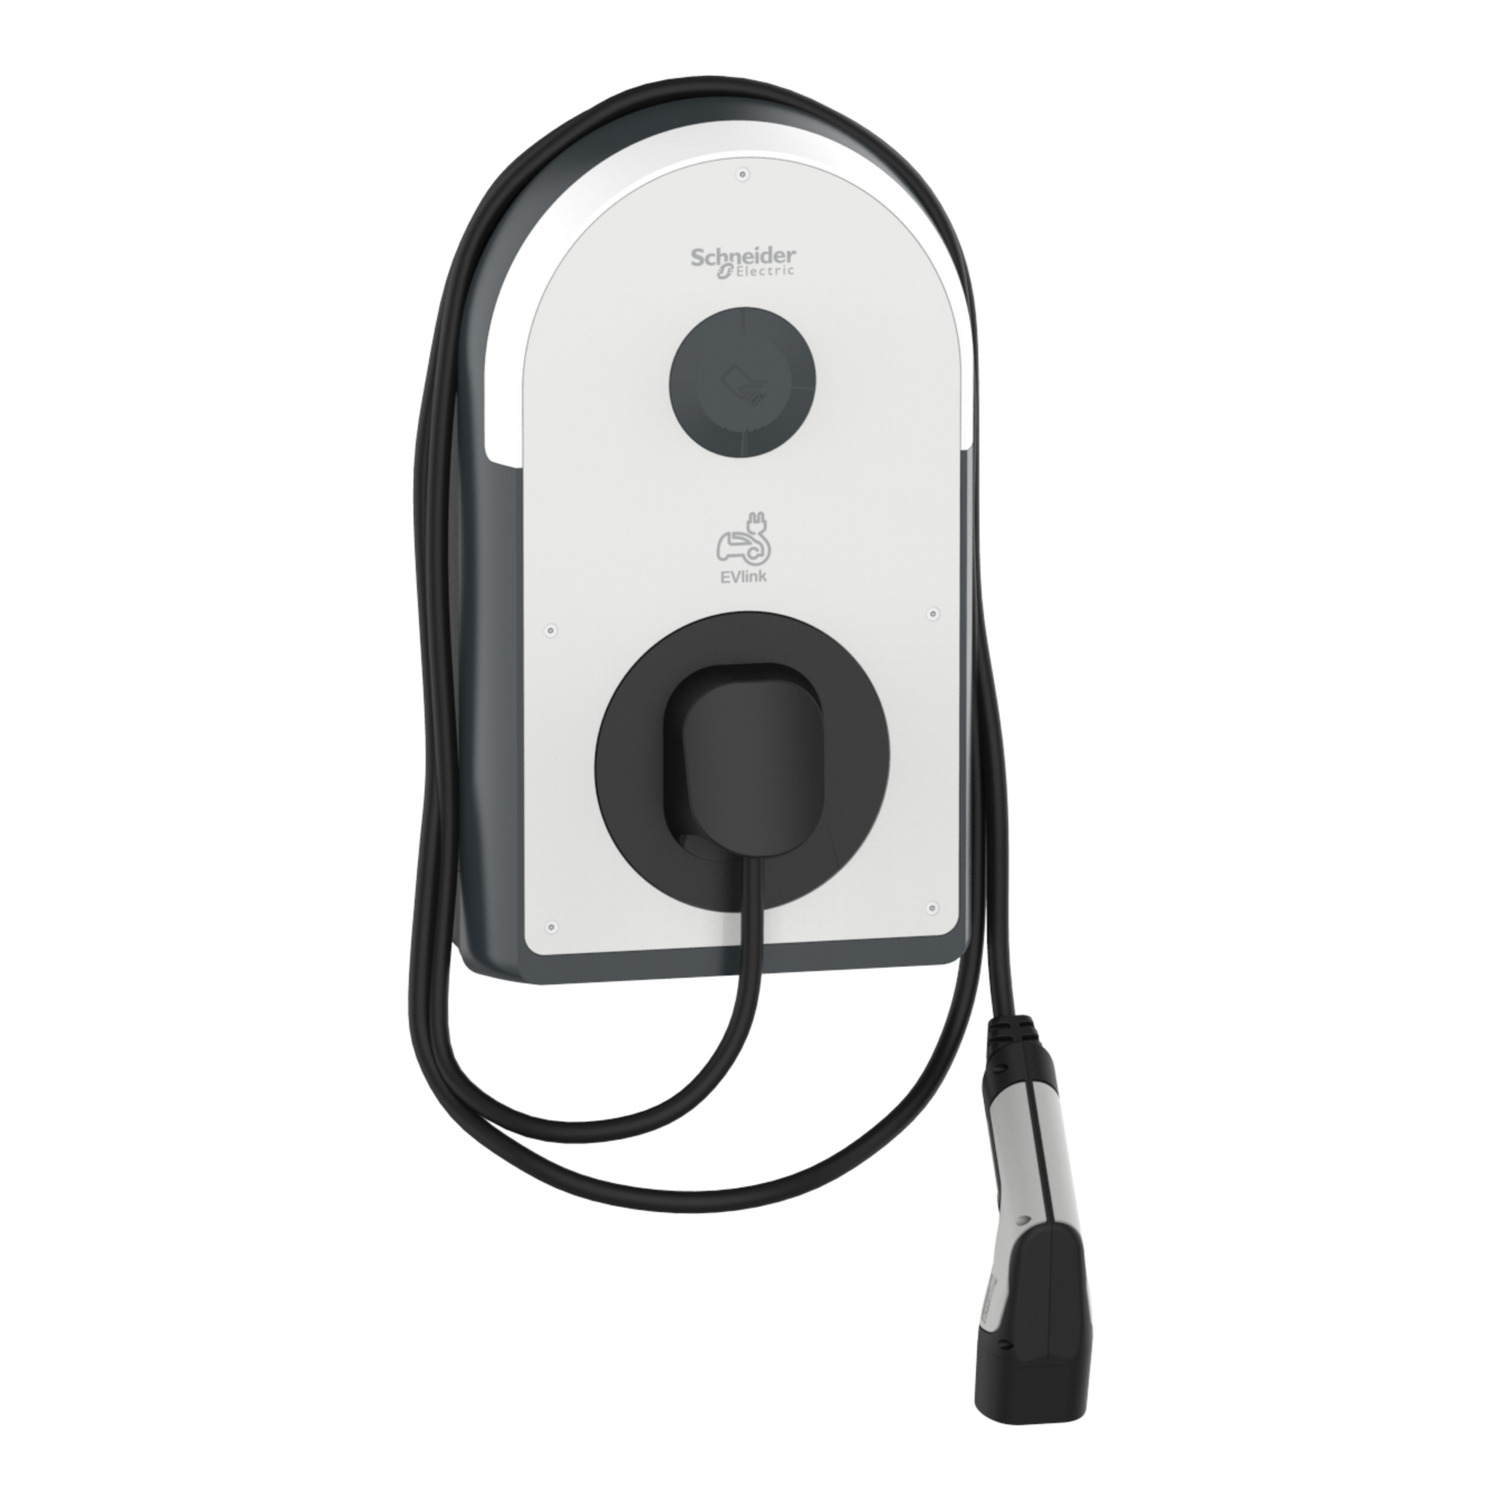
\includegraphics[width=0.5\textwidth, keepaspectratio]{figures/EVLINK.png}
    \caption{Autótöltő \cite{SE:EVLINK}} 
\end{figure}

\subsubsection{Megvalósítás}
Itt az ESP8266 firmware főbb részeit elemzem.
\paragraph{WiFi és HTTP-kiszolgáló beállítása}
Kezdésnek az ESP8266 csatlakozik WiFi-re és ezzel a helyi hálózatra a megadott SSID és jelszóval. 
A csatlakozást követően az eszköz az ESP8266WebServer könyvtár segítségével inicializál egy HTTPS-kiszolgálót. 
Ez a szerver egy kijelölt porton (pl. 8663) figyel, és a /metrics végpontot teszi közzé, 
ahol közli az adatokat a központ vezérlővel.

\subsubsection{Mérési adatok elküldése}

A \texttt{sendMetricsToEndpoint()} függvény formázza a méréseket Prometheus-szerű szöveges formába. A metrikák a következőket tartalmazzák:

\begin{itemize}
  \item \textbf{esp8266\_current0}: A mért áramértéket mutatja.
  \item \textbf{esp8266\_connection}: Az ESP8266 kapcsolati állapotát jelzi, pl.: csatlakozva vagy nem.
\end{itemize}

Ez a funkció a Prometheus-kompatibilis mért érték és címkézési formátummal küldi el a mérést. 
Amikor például a vezérlő szerver lekéri a \texttt{/metrics} végpontot, a HTTPS-kiszolgáló 
\texttt{200 OK} státusszal küldi vissza ezeket a formázott metrikákat, amennyiben minden rendben ment.

\subsubsection{Main loop}
A loop() funkcióban az ESP8266 folyamatosan kezeli a bejövő HTTPS kéréseket és 30 másodpercenként 
az eszköz meghívja a queryPrometheus() függvényt, hogy frissítse az összesített metrikát. 
Ez az időszakos lekérdezési mechanizmus biztosítja, hogy a helyi mérések folyamatosan frissek 
legyenek és döntéshozatal alapjául lehessen venni őket.

\subsubsection{Kommunikáció}
A rendszer itt is a biztonságos adatátvitel érdekében minden hálózati kommunikációhoz HTTPS protokollt használ. 
A legfontosabb adatáramlások a következők:

\begin{itemize}
    \item \textbf{Mérések közzététele:} Az ESP8266 összegyűjti az aktuális méréseket, és azokat a /metrics 
    végponton olyan formátumban teszi elérhetővé, ami már alkalmas Prometheus alapú adattárolásra.
    
    \item \textbf{Visszacsatolási hurok:} Az ESP8266 vezérlési értékeket kap a szervertől, amiket aztán modbuson 
    ad tovább az eszközöknek.
\end{itemize}

\subsubsection{Modbus kommunikáció vezérléshez}
Ez a funkció az autó töltő áramhatárának beállítására szolgál. 
Az itt használt Modbus RTU használatával az ESP8266 lesz a master, ami „Write Single Register” 
parancsot ad az autó töltőnek (Modbus slave). Az autós töltő áramkorlátja egy előre meghatározott 
regiszterben található.

\paragraph{Hardver}

\begin{itemize}
    \item \textbf{RS485:}
    Az ESP8266 natívan nem támogatja az RS485 kommunikációt, viszont tudunk használni egy RS485 adó-vevőt 
    (pl. MAX485). Ez az ESP8266 UART jeleit RS485-re alakítja, ami az ipari kommunikációban elterjedt szabvány, 
    ezért jellemzően a töltőkben és egyéb épületinformatikai eszközökben is megtalálható.
    \item \textbf{ModbusMaster könyvtár:}
    Itt az open source ModbusMaster könyvtárat \cite{ModbusMaster} használtam a továbbítás egyszerűsítésére.
    \item \textbf{Átviteli vezérlés:}
    Az előbb említett adó-vevőnek szüksége van egy úgynevezett DE/RE (Driver Enable/Receiver Enable) vezérlőpinre. 
    Amit viszont egyszerű megvalósítani az ESP8266-on egy digitális pin segítségével amire itt a D2 lett használva. 
    Ezzel tudunk később adó és vevő módok között kapcsolni. Küldéshez a pin HIGH (adási mód), ezután a 
    vételhez, pedig (vételi mód) állapotba kerül, ekkor LOW.
\end{itemize}


\subsection{Megszakító}
\subsubsection{Hardver}

A felügyelet- és vezérlésben minden megszakító egy ESP8266 modulhoz van csatlakoztatva, 
ami megkapja az aktuális állapotot, és ki-/bekapcsolást tud végezni. 
Legfontosabb komponensek és munkafolyamatok:
\begin{itemize}
    \item Állapotérzékelés: Az ESP8266 digitális bemenete a megszakító egy 
    segédérintkezőjéhez van kötve. Ha a megszakító zárva van, az érintkező bezár 
    és az ESP bemenetét magasra húzza, ha nyitva van, a bemenet alacsony. 
    Egy sima RC-szűrő és szoftveres pergésmentesítéssel (pl. 50 ms) lehet biztosítani
    a tiszta és zaj mentes átmeneteket.
    \item Parancskimenet: Egy GPIO pin egy relét húz meg, ami a megszakító 
    kioldó/becsukó tekercsét aktiválja.
\end{itemize}

\begin{figure}[!ht]
    \centering
    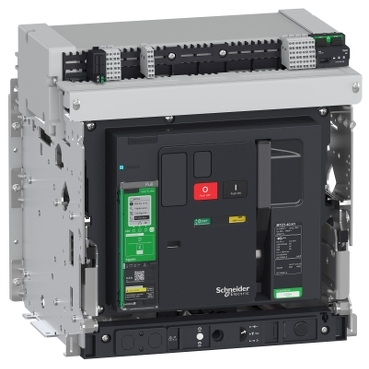
\includegraphics[width=0.5\textwidth, keepaspectratio]{figures/MTZ.jpg}
    \caption{Megszakító \cite{SE:MasterpactMTZ}} 
\end{figure}

\subsubsection{Szoftver}

Az ESP8266 arduino alapokon fut, és HTTPS segítségével csatlakozik a LAN-hoz 
Wi-Fi-n keresztül. Minden megszakító interakció RESTful API hívásokon keresztül 
történik a Python vezérlő szerverhez:

\begin{lstlisting}
    https://<control-server>/api/breakers/<id>/state
\end{lstlisting}

\begin{lstlisting}
    { "breaker_state": 1 }
\end{lstlisting}

A metrika mezők használatával a Python szerver fordítás nélkül le tudja képezni a 
bejövő JSON-t a Prometheus-nak megfelelő formátumra 
(breaker\_state és breaker\_command).

\section{Kontroll szerver}

\section{Adatbázis}

A rendszer által generált adatok tárolásához egy Prometheus adatbázist használok. 
A Prometheus egy nyílt forráskódú idősoros adatbázis, ami inkább felhő környezetben ismert, 
de ugyanolyan hasznos az IoT-telemetria számára. Minden adatot időbélyegzett értéksorozatként kezel.
Ezeket lehet tárolni és lekérdezni.
\cite{electrofunsmart:iotserver}
\cite{prometheus:dimenzionális}

Esetemben minden metrika tárhelyeként szolgál. Ez lehetővé teszi, 
hogy megőrizzem a töltési áramok történetét és ez alapján irányítsam a rendszert.

\begin{figure}[!ht]
    \centering
    
\includegraphics[width=0.5\textwidth, keepaspectratio]{figures/maxresdefault.jpg}
    \caption{Prometheus \cite{youtube:someid}} 
\end{figure}

A Flask szerver-ből könnyű továbbítani az adatokat. A megközelítés amit én használtam hogy egy HTTPS /metrics 
végpont elérhetővé tettem. Amin prometheus által olvasható formában hirdettem az adatokat. 
Például a Flask alkalmazás tudja továbbítani a mért számokat:
\begin{lstlisting}
    current_gauge = prometheus_client.Gauge('ev_charger_current', 'Current draw of EV charger', ['charger']). 
\end{lstlisting}

Ha olvasás érkezik, a szerver frissíti a számokat (egyébként ezt periodikusan is megteszi)
\begin{lstlisting}
    current_gauge.labels(charger=id).set(value). 
\end{lstlisting}

A Prometheus-nak előre megkell adni az ip-címeket a konfugorációs filejában
(a scrape konfigurációján keresztül), hogy időszakonként megnézze a Flask szerver 
/metrics URL-jét. 
Ez azért előnyösebb mert utólag ezeket már nem lehet állítani a prometheusban indítás után.
A szerver, pedig egy stabil IP címen van. A sok fizikai végpontról, pedig a szerver gyújt ahol elértem, hogy 
üzem közben is lehessen új végpontokat hozzáadni vagy módosítani.

Amikor a Prometheus olvas, a Flask az összes aktuális értéket szöveges 
Prometheus metrika formátumban adja ki. A Prometheus ezután ezeket az értékeket a metrikanévvel és címkékkel 
indexelve tárolja. Ez a lehívás alapú felügyelet jól illeszkedik a Prometheus működéséhez. 
A Prometheus adatai megjeleníthetők a Grafana által is és összetett lekérdezések írhatók 
például a teljes áram kiszámítására, amihez szükségem is volt nekem rendszer irányítsásához.

\subsection{Prometheus adatgyűjtés kezelése}

A mikrokontroller több metrikát is mér, 
amit belső változókba elment. Jelenleg teszt célokból ezek, csak kézzel megadott számok.

\begin{lstlisting}[language=HTML]
    {
      "# HELP": "esp8266_current Current sensor reading.",
      "# TYPE": "esp8266_current gauge",
      "esp8266_current0": 1.20,
      "esp8266_current1": 2.50
    }
\end{lstlisting}

Ez a formátum megengedi, hogy ezt a /metrics endpointon a prometheus folyamatosan lekérdezze a mikrokontrollerektől. \\

A formátumot a következő függvény hozza létre és küldi:

\begin{lstlisting}[language=C]
    sendMetricsToEndpoint()
    ...
    server.send(200, "text/plain", metrics);
\end{lstlisting}

\subsection{Prometheus lekérdezések kezelése}

\begin{lstlisting}[language=C]
    queryPrometheus()
\end{lstlisting}

Ez a függvény egy HTTP GET kérést küld a Prometheus szervernek, amely a esp8266\_total\_current 
metrikát kérdezi le és a prometheusValue változóba írja be.

\begin{lstlisting}
    /api/v1/query?query=esp8266_total_current
\end{lstlisting}

A fentebbi endpointon. \\
A lekérdezés sikerességét a httpCode ellenőrzésével teszem amennyiben ez 200-at ad vissza az értéket eltárolom 
és kiírom a soros kommunikáción ellenőrzés céljából.

\begin{lstlisting}[language=C]
    if (httpCode == HTTP_CODE_OK) {
      String payload = http.getString();
      Serial.println("Response from Prometheus:");
      Serial.println(payload);  \texttt{Adat JSON-be nyomtatása}

      DynamicJsonDocument doc(1024);
      DeserializationError error = deserializeJson(doc, payload);

      if (error) {
        Serial.print(F("JSON deserialization failed: "));
        Serial.println(error.c_str());
        return;
      }
    }
\end{lstlisting}

Mivel a lekérdezés egy JSON formátumú változót ad vissza és ennek feldolgozása nehézkes ezért ezt rögtön szám 
formátumba alakítom későbbi feldolgozás céljából.

\begin{lstlisting}[language=C]
    
    const char* status = doc["status"];
    if (String(status) == "success") {
      
      const char* valueStr = doc["data"]["result"][0]["value"][1];
      
      prometheusValue = String(valueStr).toFloat();

      Serial.print("Extracted Prometheus Value: ");
      Serial.println(prometheusValue);
    }
\end{lstlisting}

A fenti rész kinyeri az adatot JSON formátumból és szám formátumba írja.\\
\\
Természetesen az egész queryPrometheus loop-ban ismétlődve fut, hogy a kontroller folyamatosan frissítse az értékeket. 
Jelenleg a gyakoriságot 30 másodpercre állítottam, hogy ne terhelje a próbák során feleslegesen a hálózatot, 
de gyorsabb válaszidő érdekében ez növelhető.

\section{Grafana alapú megjelenítés}

A szerver automatikusan beavatkozik szükséges esetben, viszont emellett továbbra 
is szükséges a működtető személyzetnek látnia, a rendszer működését. Ezt folyamatosan 
ellenőrizni és amennyiben nem megfelelő működés lép fel. Akár nem működik az 
automatizmus akár rosszul működik, szükséges beavatkozni manuálisan.

\subsection{A háromfázisú és a napelemes áram vizualizálása és riasztása a Grafanában}
Ebben a fejezetben bemutatom, hogy a nyers árammérések az egyes EV-töltők és 
egyéb terhelések hogyan oszlanak meg három fázison, valamint a napelemek 
bemeneti áramai hogyan jelennek meg Grafanában, és hogyan történik a 
túláram vagy más veszélyes állapotok automatikus vagy manuális kezelése. 
Minden eszköz a Prometheus metrikákat exportálja a következőképpen:

\begin{lstlisting}
ev_charger_current_phase_a_amplitude{charger="ev1"} 12.3
ev_charger_current_phase_b_amplitude{charger="ev1"} 11.8
ev_charger_current_phase_c_amplitude{charger="ev1"} 12.1

equipment_current_phase_a_amplitude{device="pump1"} 5.4
... 

solar_input_current_amplitude 8.7
\end{lstlisting}

\subsubsection{A Dashboard}
\paragraph{1. sor}
EV töltők áramai amik a
\$charger változóval vannak jelölve, ez felsorolja az összes ide  tartozó cimke értékét 
(pl. „ev1”, „ev2”, ...).
Ezután az idősoros panel: ábrázolja az összegzett értéket három fázison.
\begin{lstlisting}
    ev_charger_current{charger="$charger"}
\end{lstlisting}
Itt ugyanazon a tengelyen láthatóak a három fázis összegzett értékei, 
különböző színnel és elnevezéssel.
Az úgynevezett "mérőpanelen" a pillanatnyi fázisáramokat három kis mérő formájában
lehet látni igazából továbbra is a a fenti lekérdezésseket használva, 
pillanatnyi csak üzemmódban.
A küszöb értékeket állítottam be a könnyeb vizualizáció érdekében 
a töltő névleges áramának, 
80 \%-ánál (sárga) és 100 \%-ánál (piros) vannak beállítva.

\paragraph{2. sor}
Segédberendezések áramai
A \$device változóban keressük ezeket a metrikákat.

A panel hasonlóan az előző ponthoz jeleníti meg az adatokat, amely a pillanatnyi 
és max értéket mutatja.
\begin{lstlisting}
    max_over_time(equipment_current_phase_a_amplitude{device="\$device"}[1m])
\end{lstlisting}
A maximumot minden fázisra az elmúlt percben mutatja, az idetartozó 
megfelelő színküszöbökkel.
Mellette raktam egymás mellé csoportosító oszlopdiagramot a gyors 
összehasonlításokra.

\paragraph{3. Sor}
Napelem bemeneti áram
Itt szintén egy idősoros panelt alkalmaztam a megjeleníthetőség érdekében.
\begin{lstlisting}
    solar_input_current_amplitude
\end{lstlisting}

\begin{figure}[!ht]
    \centering
    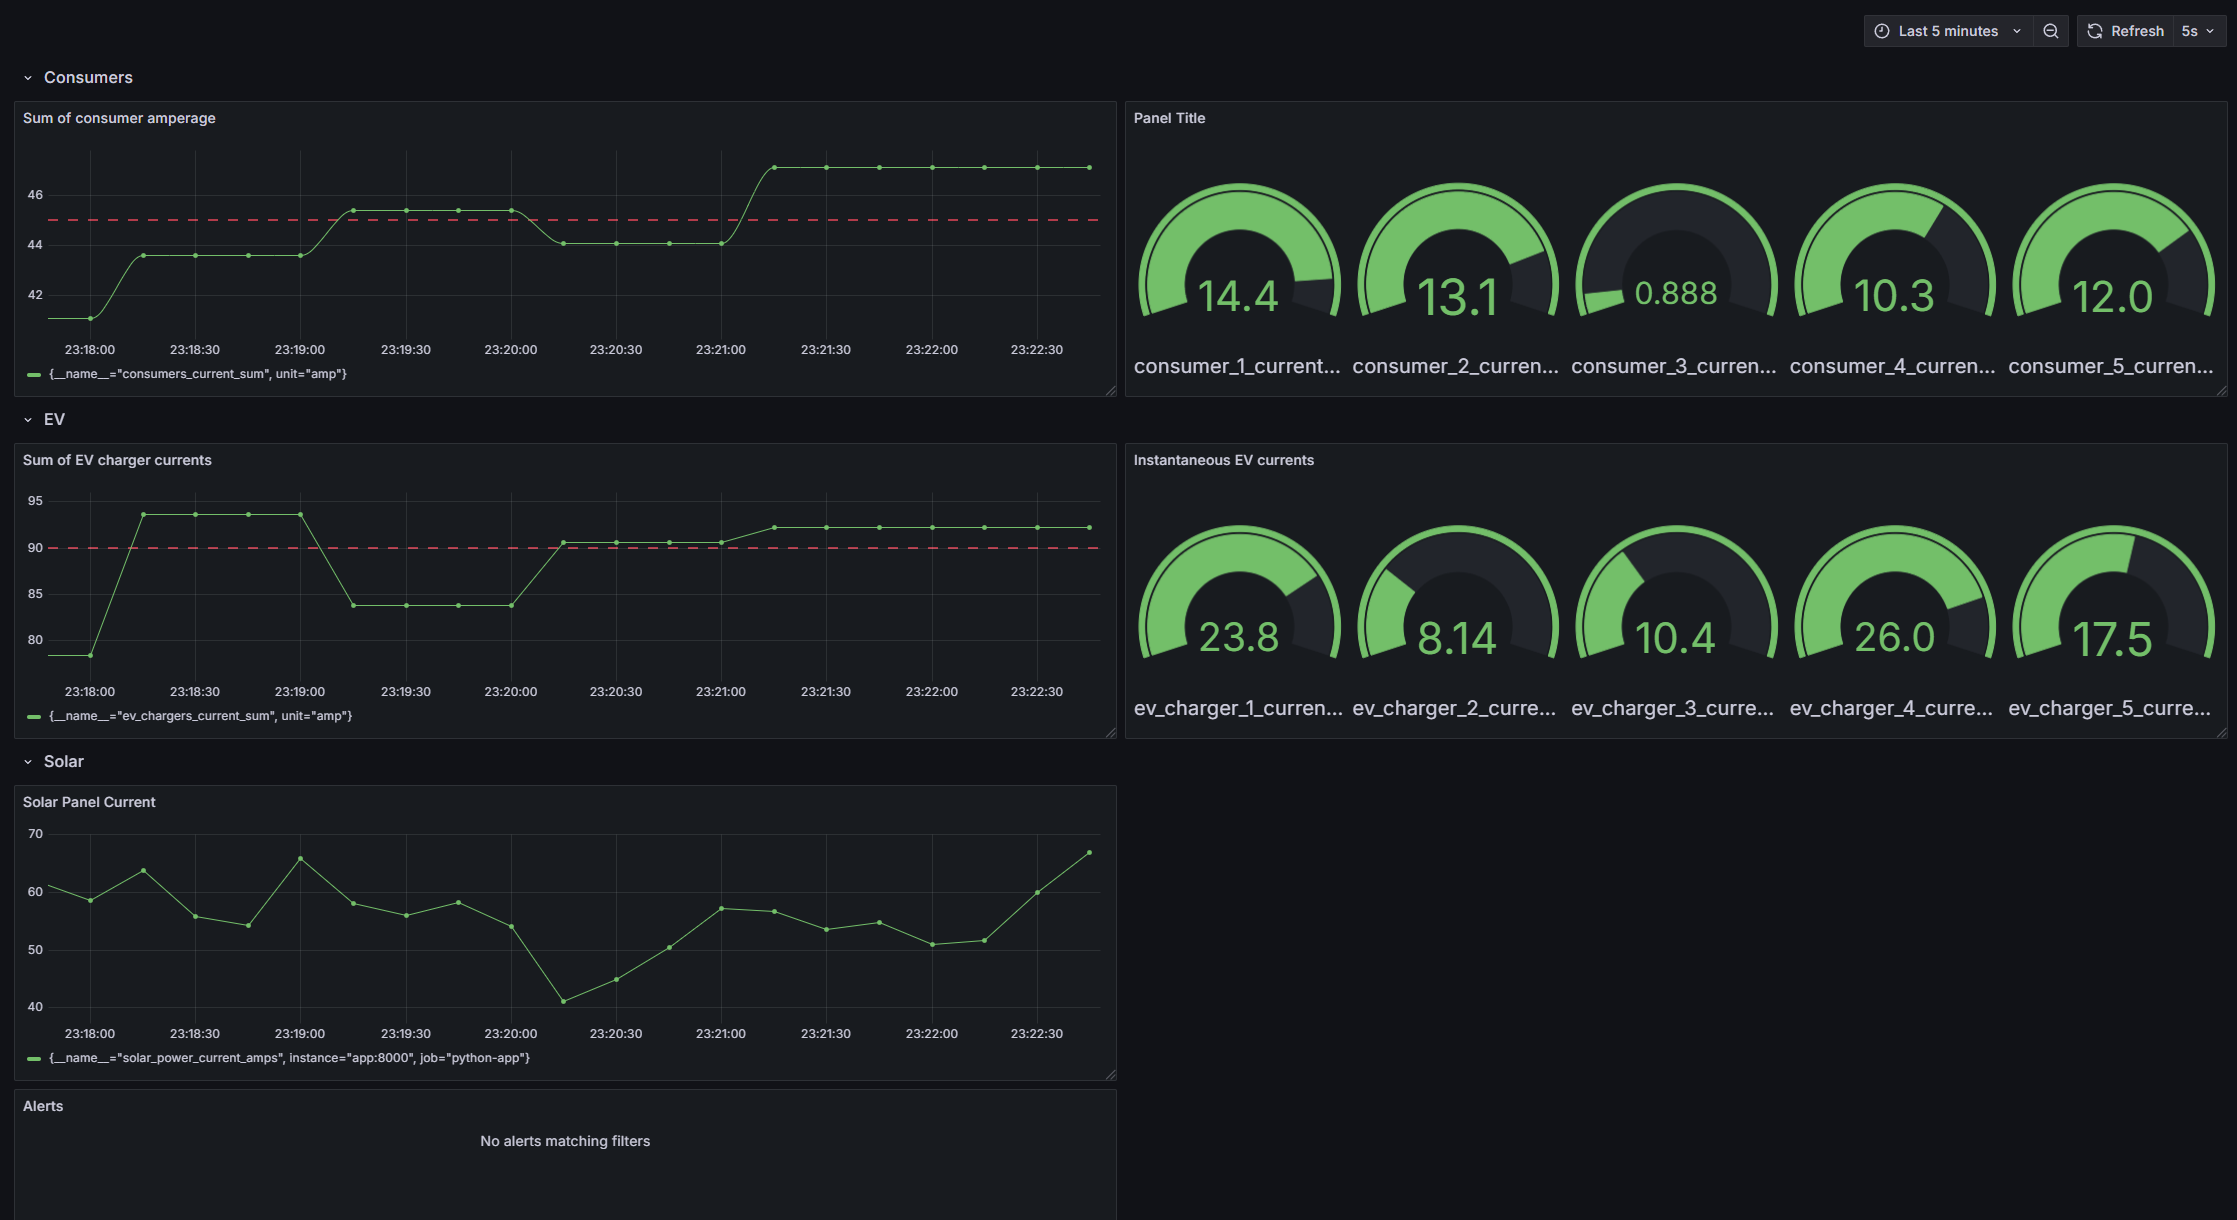
\includegraphics[width=1\textwidth, keepaspectratio]{figures/Grafana.png}
    \caption{Általam készített Grafana dashboard} 
\end{figure}